\documentclass{InsightArticle}

\usepackage[dvips]{graphicx}
\usepackage{float}
\usepackage{subfigure}
\usepackage{nicefrac}
\usepackage{amsmath,amssymb}
\usepackage[dvips,
bookmarks,
bookmarksopen,
backref,
colorlinks,linkcolor={blue},citecolor={blue},urlcolor={blue},
]{hyperref}
\newcommand{\M}[1]{\mathbf{#1}}
\newcommand{\V}[1]{\mathbf{#1}}
\newcommand{\X}{XXXXXXXXXXXXX}
\title{Hough Transform Plane Detector}

% 
% NOTE: This is the last number of the "handle" URL that 
% The Insight Journal assigns to your paper as part of the
% submission process. Please replace the number "1338" with
% the actual handle number that you get assigned.
%
\newcommand{\IJhandlerIDnumber}{3290}

% Increment the release number whenever significant changes are made.
% The author and/or editor can define 'significant' however they like.
\release{0.00}

% At minimum, give your name and an email address.  You can include a
% snail-mail address if you like.

\author{Dorit Borrmann and David Doria}
%\authoraddress{Rensselaer Polytechnic Institute, Troy NY \and Jacobs University}


\begin{document}

\IJhandlefooter{\IJhandlerIDnumber}


\ifpdf
\else
   %
   % Commands for including Graphics when using latex
   % 
   \DeclareGraphicsExtensions{.eps,.jpg,.gif,.tiff,.bmp,.png}
   \DeclareGraphicsExtensions{.png,.bb}
   \DeclareGraphicsRule{.jpg}{eps}{.jpg.bb}{`convert #1 eps:-}
   \DeclareGraphicsRule{.gif}{eps}{.gif.bb}{`convert #1 eps:-}
   \DeclareGraphicsRule{.tiff}{eps}{.tiff.bb}{`convert #1 eps:-}
   \DeclareGraphicsRule{.bmp}{eps}{.bmp.bb}{`convert #1 eps:-}
   \DeclareGraphicsRule{.png}{eps}{.png.bb}{`convert #1 eps:-}
\fi


\maketitle


\ifhtml
\chapter*{Front Matter\label{front}}
\fi

\begin{abstract}
\noindent
This document presents a VTK wrapper of an extracted portion of `3DTK - The 3D Toolkit' (http://threedtk.de) to enable a developer to find planes in 3D point cloud data.

\vspace{14pt}

\noindent The code is available at:

\noindent
http://sourceforge.net/projects/slam6d/files/3dtk-houghplanes-for-vtk-release-1.0.tgz/download
%https://github.com/daviddoria/VTKHoughPlanes

\end{abstract}

\IJhandlenote{\IJhandlerIDnumber}

\tableofcontents

%%%%%%%%%%%%
\section{Introduction}
Finding planes in 3D point clouds is a very common operation. This code uses the
Hough Transform to find the strongest planes in a point cloud and then labels
each point with the label of the plane to which it belongs. The methods
implemented in 3DTK are explained in detail in~\cite{Borrmann:2011}. A very
brief description is also given in the following section. For a more detailed view please refer to
the original article.

%%%%%%%%%%%%
\section{The Hough Transform}

\begin{figure}[H]
\centering
\subfigure[Polar coordinates of normal vector]{
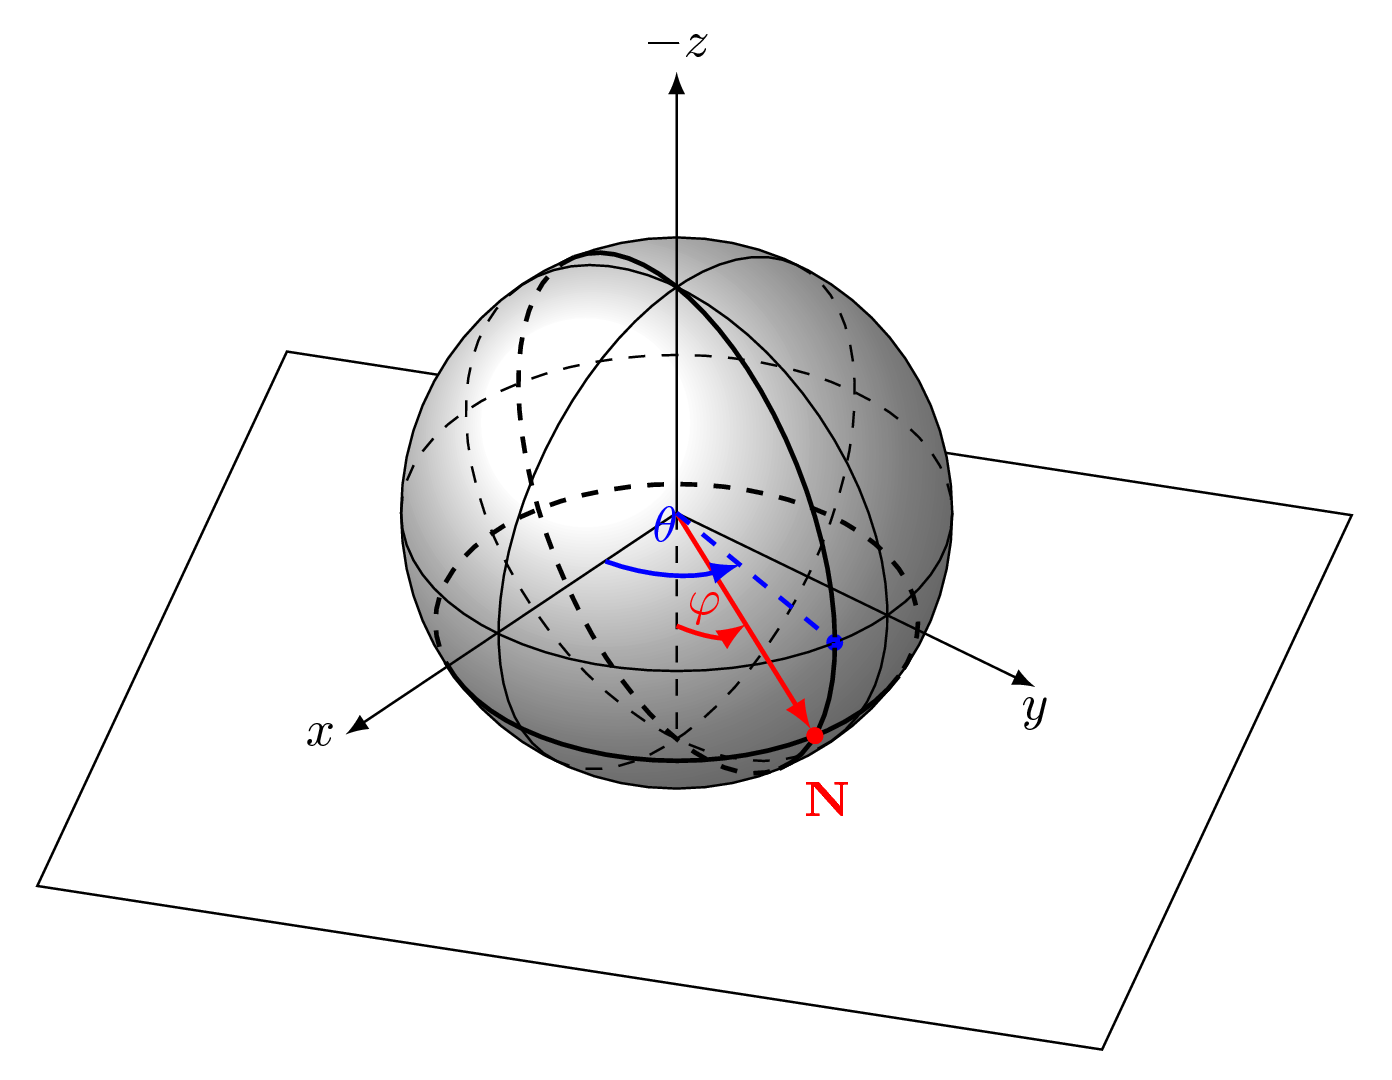
\includegraphics[width=0.33\textwidth]{images/polar1}
\label{fig:polar}
}
\subfigure[Hough Transform of $3$ points] {
\includegraphics[width=0.33\textwidth]{images/hough3}
\label{fig:sinusoid}
}
\subfigure[Accumulator] {
\includegraphics[width=0.25\textwidth]{images/accumulator}
\label{fig:accumulator}
}
\caption{The Hough Transform.}
\end{figure}

The Hough Transform \cite{Hough:1962, Duda:1971} is a method for detecting parametrized
objects. In this software package it is used to detect planes in 3D point
clouds. A plane is typically represented by its normal vector $\V{n}$ and the
distance $\rho$
from the origin. Let $\theta$ be the angle of the normal vector on the
$xy$-plane and $\varphi$ the angle between the $xy$-plane and the normal vector
in $z$ direction (cf. Figure~\ref{fig:polar}). Then the plane is given by 
\begin{align*}
\rho = \V{p} \cdot \V{n} = 
{p}_x \cdot \cos{\theta} \cdot \sin{\varphi} + {p}_y \cdot \sin{\varphi} \cdot
\sin{\theta} + {p}_z \cdot \cos{\varphi}
\end{align*}
for every point $\V{p}$ on the plane.
$\varphi$, $\theta$ and $\rho$ define the 3-dimensional Hough Space
($\theta,\varphi,\rho$). Each point in the Hough Space corresponds to one
\emph{plane} in $\mathbb{R}^3$. 
The Hough Transform of a point in $\mathbb{R}^3$
is a 3D sinusoid curve in Hough Space as shown in Figure~\ref{fig:sinusoid}. The point in Hough Space where the
curves for three points intersect corresponds to the plane spanned by these three
points. The more curves intersect in one point, the better this plane is
represented by the point set. 

To find planes in the point set, the Hough
Space is discretized into a so-called accumulator. Different ways of discretizing the Hough Space are
presented in \cite{Borrmann:2011}. One way is depicted in
Figure~\ref{fig:accumulator}.
Transforming a point $\V{p}$ into Hough Space means increasing the counter for all cells in the accumulator
that represent a plane through $\V{p}$. The cell with the highest
counter corresponds to the plane that is best represented by the point set.

\subsection{Hough Methods}
Applying the Hough Transform to a large point set with a fine discretization of
the Hough Space is computationally expensive. To overcome this issue there are
different variations of the Hough Transform.
\begin{description}
\item[Standardized Hough Transform (SHT)] For all points from the input point
set the complete Hough Transform is performed. Therefore this method is
deterministic. After the voting phase the cells with the maximum votes are
considered as plane candidates.
\item[Randomized Hough Transform (RHT)] Instead of performing the complete Hough
Transform for the points triples of points are randomly selected and
only the counter for the cell corresponding to the plane spanned by these points
is incremented. Whenever one counter exceeds a threshold the points
on the plane represented by this cell are removed from the point set. This
procedure typically leads to more stable results.
\item[Probabilistic Hough Transform (PHT)] The complete Hough Transform is only
performed for $p$ percent of the points from the input set. $p$ has to be
determined based on the expected noise level of the point set, e.g., the
percentage 
of points that
belong to no plane.
\item[Progressive Probabilistic Hough Transform (PPHT)] The complete Hough
Transform is performed for randomly selected points from the input set. A
threshold is calculated based on the number of points that have already voted.
Once the counter of a cell exceeds this threshold the voting phase is stopped and
the points that lie on the corresponding plane are deleted. This algorithm is less sensitive to noise in the data.
\item[Adaptive Probabilistic Hough Transform (APHT)] Sets of 10 points are
randomly selected from the input point set. For these points the complete Hough
Transform is performed. A list of maxima is maintained and updated after each
voting round. Based on the stability of this list plane candidates are
selected.
\end{description}
\section{Demonstration}
Figure~\ref{fig:Demonstration} demonstrates the algorithm.
Figure~\ref{fig:Demonstration:InputPoints} shows a LiDAR scan of a flat panel
monitor sitting on a counter. Figure~\ref{fig:Demonstration:OutputPoints} shows the points colored by the plane to which they belong.

\begin{figure}[H]
\centering
\subfigure[Input points.]
  {
  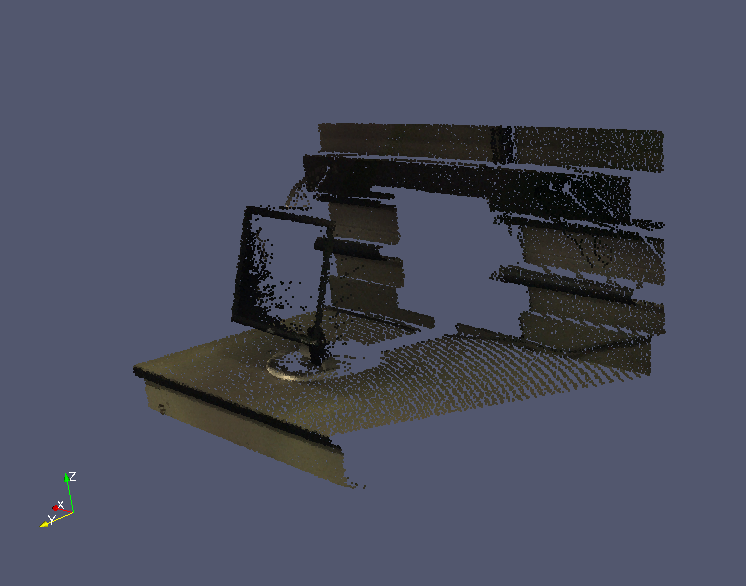
\includegraphics[width=0.3\linewidth]{images/counter}
  \label{fig:Demonstration:InputPoints}
  }
\subfigure[Output points.]
  {
  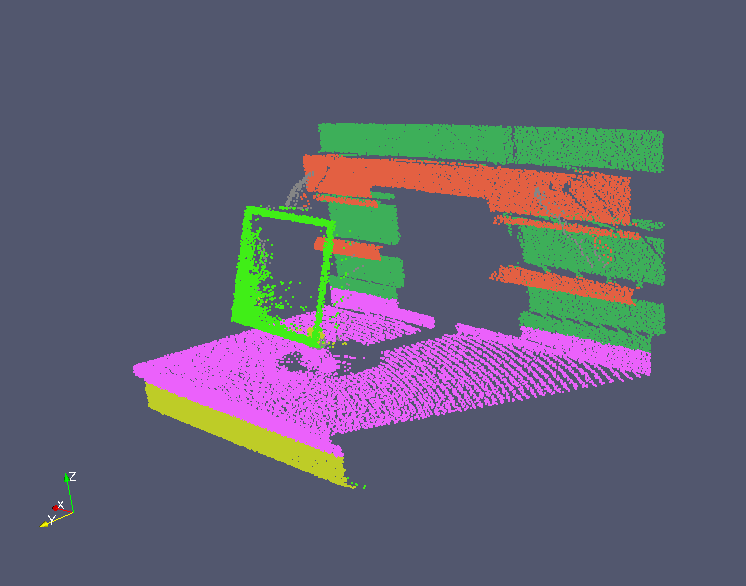
\includegraphics[width=0.3\linewidth]{images/counterPlanes}
  \label{fig:Demonstration:OutputPoints}
  }
\caption{Demonstration}
\label{fig:Demonstration}
\end{figure}

\subsection{Code Snippet}
The vtkHoughPlanes class must be passed an input vtkPolyData via SetInputConnection. The many parameters can also be set as demonstrated below.
\begin{verbatim}
  // Read the input file
  vtkSmartPointer<vtkXMLPolyDataReader> reader =
    vtkSmartPointer<vtkXMLPolyDataReader>::New();
  reader->SetFileName(inputFileName.c_str());
  reader->Update();
  
  vtkSmartPointer<vtkHoughPlanes> houghPlanes =
    vtkSmartPointer<vtkHoughPlanes>::New();
  houghPlanes->SetInputConnection(reader->GetOutputPort());
  houghPlanes->SetMaxDist(2.00);
  houghPlanes->SetMinDist(0.10);
  houghPlanes->SetAccumulatorMax(100);
  houghPlanes->SetMinSizeAllPoints(5);
  houghPlanes->SetRhoNum(100);
  houghPlanes->SetThetaNum(360);
  houghPlanes->SetPhiNum(176);
  houghPlanes->SetRhoMax(5.00);
  houghPlanes->SetMaxPointPlaneDist(0.050);
  houghPlanes->SetMaxPlanes(30);
  houghPlanes->SetMinPlaneSize(100);
  houghPlanes->SetMinPlanarity(0.300);
  houghPlanes->SetPlaneRatio(0.5);
  houghPlanes->SetPointDist(0.050);
  houghPlanes->SetPeakWindow(false);
  houghPlanes->SetWindowSize(8);
  houghPlanes->SetTrashMax(20);
  houghPlanes->SetAccumulatorType(1);
  houghPlanes->SetHoughAlgorithm(vtkHoughPlanes::Randomized);
  houghPlanes->Update();

  // Write output points colored by plane
  vtkSmartPointer<vtkXMLPolyDataWriter> writer = 
    vtkSmartPointer<vtkXMLPolyDataWriter>::New();
  writer->SetInputConnection(houghPlanes->GetOutputPort());
  writer->SetFileName(outputFileName.c_str());
  writer->Write();

\end{verbatim}


\newenvironment{liste}[2][\rm]{\begin{list}{}{\settowidth{\labelwidth}{{#1#2}}
  \setlength{\leftmargin}{\labelwidth}\addtolength{\leftmargin}{\labelsep}
    \addtolength{\leftmargin}{0ex}%changed from 3 to 0
      \setlength{\parsep}{.5ex plus0.2ex minus 0.2ex}%
        \setlength{\itemsep}{1ex}%
          \renewcommand{\makelabel}[1]{{#1##1\hfill}}}}
            {\end{list}}%

\subsection{Explanation of parameters}

The Hough Transform needs many parameters to fine tune the application. The
implementation does not depend on any unit of measurement. However, it is
indispensible that the units of the parameters match with the units used for the input data.

General parameters:
\begin{liste}{\X}
\item[\texttt{AccumulatorType}] The software offers different accumulator
types: 
\begin{enumerate}
\item[1:] the Accumulator Array with a linear discretization of the Hough Space,
\item[2:] the Accumulator Ball with similar cell sizes when the Hough Space is mapped
onto the unit sphere, 
\item[3:] the Accumulator Cube where the discretization is based
on projecting a cube onto the unit sphere, 
\item[4:] the improved Accumulator Ball,
where each of the two poles is represented by a single cell.
\end{enumerate}
\item[\texttt{HoughAlgorithm}] The implemented Hough variations are are SHT,
RHT, PHT, PPHT, and APHT.
\end{liste}

The different Hough methods have various stopping rules. The following
parameters are used to define the thresholds for these stopping rules:
\begin{liste}{\X}
\item[\texttt{MinSizeAllPoints}] Defines a threshold when to stop applying
the Hough Transform. The number indicates the percentage of points from the
input point cloud that have not been asigned to a plane.
\item[\texttt{MaxPlanes}] Defines a threshold for the maximum number of planes that
are detected.
The algorithms stops after this amount of planes has been reached.
\item[\texttt{TrashMax}] Threshold that defines after how many discarded
planes the algorithm is stopped. If one cell in the accumulator receives enough
votes, a plane is fitted through all points that
belong to the represented plane. Planes are discarded if they are only
represented by a small number of points, or if the planarity of the sample
points is too low.
\end{liste}

For practical applications the Hough Space is discretized. The following
parameters define the discretization:

\begin{liste}{\X}
\item[\texttt{RhoMax}] Defines the maximum distance $\rho_{max}$ of a plane from the origin for
discretization.
\item[\texttt{RhoNum}] Defines the number of cells $\rho_{N}$ in direction of $\rho$. Each cell
has the size $\nicefrac{\rho_{max}}{\rho_{N}}$.
\item[\texttt{ThetaNum}] Defines the number of cells $\theta_{N}$ in direction of $\theta$.
\item[\texttt{PhiNum}] Defines the number of cells $\varphi_{N}$ in direction of $\varphi$. Each
cell has the size $\nicefrac{\varphi_{N}}{\varphi_{N}}$. 
\end{liste}

Plane parameters:

\begin{liste}{\X}
\item[\texttt{MaxPointPlaneDist}] Maximal distance between a point and the
plane so that the point is still considered to belong to the plane. This
parameter is used to compensate measurement noise and discretization.
\item[\texttt{MinPlanarity}] A detected plane is discarded if the planarity
falls below this threshold. Each plane candidate is fitted through all points
that are considered to belong to it using a least squares method based on the
Jacobi eigenvalue algorithm. The planarity is given by the value of the smallest
eigenvalue devided by the number of points.
\end{liste}

Additional parameters for certain algorithms:

\begin{liste}{\X}
\item[\texttt{PlaneRatio}] For the SHT and the PHT the maxima in the
accumulator are determined after the accumulation phase is completed. The
\texttt{PlaneRatio} is a threshold $r$ that determines which maxima from the
accumulator are considered to be detected planes. Each cell in the accumulator
with a count lower than $r\cdot max_c$ is discarded, where $max_c$ is highest score
in the accumulator
\item[\texttt{PeakWindow}] For the SHT and the PHT the maxima in the
accumulator are determined after the accumulation phase is completed. If
\texttt{PeakWindow} is set to false the raw maxima in the accumulator are used,
otherwise a sliding window technique is used to filter out maxima in the
accumulator that are close to each other.
\item[\texttt{WindowSize}] Sets the side lenght of the sliding window for
peak detection.
\end{liste}

\begin{liste}{\X}
\item[\texttt{MinDist}] Sets the minimum distance for the three points
selected to calculate the model plane for the Randomized Hough Transform.
\item[\texttt{AccumulatorMax}] Sets the maximum distance for the three points
selected to calculate the model plane for the Randomized Hough Transform.

\end{liste}

\bibliographystyle{plain}
\bibliography{papers}

\end{document}
